\documentclass[ngerman,xcolor=svgnames]{beamer}
% colors: http://www.math.umbc.edu/~rouben/beamer/quickstart-Z-H-25.html#node_sec_25

\usepackage[german]{babel}
\usepackage[T1]{fontenc}
\usepackage{graphicx}
\usepackage{ifthen}
\usepackage{listings}
\usepackage{verbatim}
\usepackage{fancyhdr}
\usepackage{tikz}
\usepackage{dsfont}
\usetikzlibrary{spy,matrix}
\usepackage[style=mla, backend=bibtex]{biblatex}
\bibliography{storm}

\usepackage{xunicode}
\usepackage{xltxtra}
\usepackage{setspace}
\defaultfontfeatures{Mapping=tex-text}
\setmonofont[Mapping={}, Scale=MatchLowercase]{DejaVu Sans Mono}
\setsansfont[Scale=MatchLowercase]{Linux Biolinum O}
\setmainfont[]{Linux Libertine O}

\newbox\mytempbox
\newdimen\mytempdimen
\newcommand\includegraphicscopyright[3][]{%
  \leavevmode\vbox{\vskip3pt\raggedright\setbox\mytempbox=\hbox{%
  \includegraphics[#1]{#2}}%
    \mytempdimen=\wd\mytempbox\box\mytempbox\par\vskip1pt%
    \fontsize{3}{3.5}\selectfont{\color{black!25}{\vbox{\hsize=\mytempdimen#3}}}\vskip3pt%
}}

\newcommand\prelim[1]{\small }

\newcommand\strColor[1]{\color{beamer@blendedblue}{#1}}

\newcommand\sect[1]{\begin{center}\huge\strColor{#1}\end{center}}

\setbeamertemplate{navigation symbols}{}

\pagestyle{fancy}
\rhead{\vspace{.3em}
\includegraphics[width=10em]{assets/FULogo_RGB.eps}}
\cfoot{}
\renewcommand{\headrulewidth}{0pt}

\lstset{language=C}
\lstset{basicstyle=\tiny\ttfamily}
\lstset{breaklines=true}
\lstset{keywordstyle=\color{purple}}

\usepackage{geometry}
\usepackage{tikz}
\usetikzlibrary{calc,arrows}

\newdimen\XCoord
\newdimen\YCoord

\newcommand*{\ExtractCoordinate}[1]{\path (#1); \pgfgetlastxy{\XCoord}{\YCoord};}%

\title{Gossiping on Mobile Devices}
\author{Michael Krause, Robin Nehls, Jakob Pfender}
\institute{FU Berlin\\Institut für Informatik\\Softwareprojekt
Mobilkommunikation}
\date{11. Februar 2014}

\begin{document}

\frame{\titlepage}

\frame{
  \huge{Recap}

}

\frame{
\frametitle{Recap}
\begin{itemize}
  \item \textbf{Our goals:}
    \begin{itemize}
      \item Application layer gossiping for keeping information in
        a (P2P) network
      \item Implementation on an embedded board, using RIOT
      \item Visualization using LEDs
    \end{itemize}
  \item \textbf{Our ideas:}
    \begin{itemize}
      \item Implement gossiping as infrastructure for other applications
      \item Leader election using gossiping infrastructure
      \item Time synchronization using leader election \& gossiping
    \end{itemize}
\end{itemize}
}

\frame{
    \frametitle{Recap -- Gossip implementation}
    \begin{itemize}
      \item Nodes assign themselves random IDs, announce their presence,
        build neighbour tables and start gossiping messages to random
        neighbours
      \item Neighbour tables are kept up to date with cleanup functions
        and reannouncements
    \end{itemize}
}

\frame{
    \frametitle{Recap -- Leader election}
    \begin{itemize}
      \item If a node doesn't know who the leader is, it elects itself
      \item If a node receives a leader ID that's ``better`` than the
        one it currently knows, it adapts that leader as new leader
      \item If a node receives a leader ID that's ``worse`` than the one it
        currently knows, it immediately replies with its own leader
      \item Leader information is thus disseminated through the network
        via gossiping
      \item Nodes always behave as if their locally known leader is the
        true leader
    \end{itemize}
}

\begin{frame}[fragile]
  \frametitle{Leader election -- example}
  \begin{center}
    \includegraphics<1>[scale=0.2]{assets/network_01}
    \includegraphics<2>[scale=0.2]{assets/network_02}
    \includegraphics<3>[scale=0.2]{assets/network_03}
    \includegraphics<4>[scale=0.2]{assets/network_04}
    \includegraphics<5>[scale=0.2]{assets/network_05}
    \includegraphics<6>[scale=0.2]{assets/network_06}
    \includegraphics<7>[scale=0.2]{assets/network_07}
    \includegraphics<8>[scale=0.2]{assets/network_08}
    \includegraphics<9>[scale=0.2]{assets/network_09}
    \includegraphics<10>[scale=0.2]{assets/network_10}
    \includegraphics<11>[scale=0.2]{assets/network_11}
    \includegraphics<12>[scale=0.2]{assets/network_12}
    \includegraphics<13>[scale=0.2]{assets/network_13}
    \includegraphics<14>[scale=0.2]{assets/network_14}
  \end{center}
\end{frame}


\frame{
  \huge{Time synchronization}

}

\frame{
    \frametitle{Time synchronization}
    \begin{itemize}
      \item If a node is the current leader or has received its
        timestamp from the leader (directly or indirectly), it may
        initiate time synchronization
      \item Current timestamp is gossiped to a random neighbor
      \item Upon reception of a timestamp, a node records the time of
        reception and replies with a \lstinline!DELAYREQ! message
      \item Upon reception of a \lstinline!DELAYREQ!, the master once
        again records the current time and sends it back with
        a \lstinline!DELAYRESP! message
      \item Upon reception of a \lstinline!DELAYRESP!, a node records
        the time of reception
      \item Using these four timestamps, the node can calculate its
        offset to the master and adjust its own clock accordingly
    \end{itemize}
}

\frame{
    \frametitle{Time synchronization}
    \begin{center}
        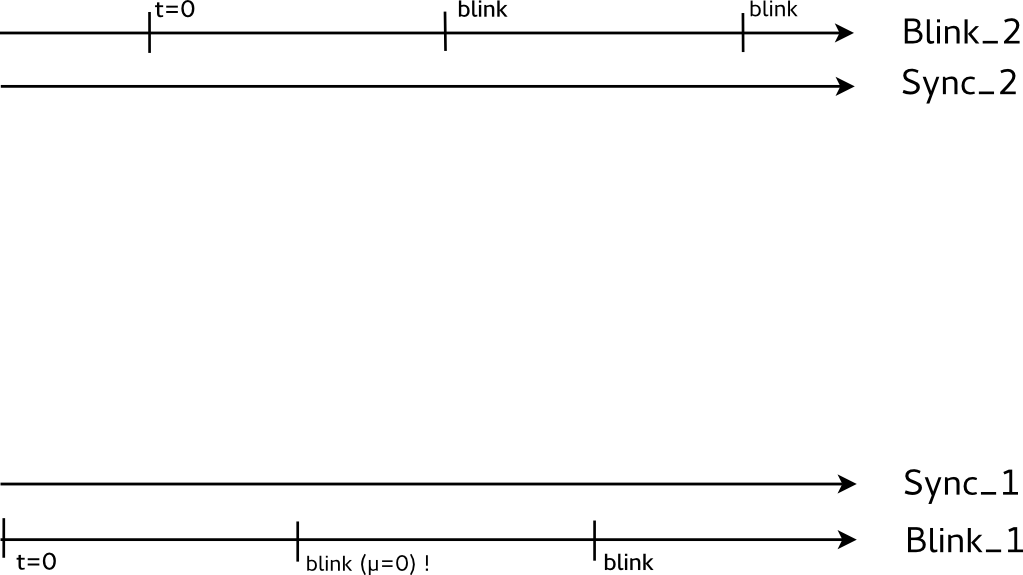
\includegraphics[scale=0.35]{assets/timesync-1.png}
    \end{center}
}
\frame{
    \frametitle{Time synchronization}
    \begin{center}
        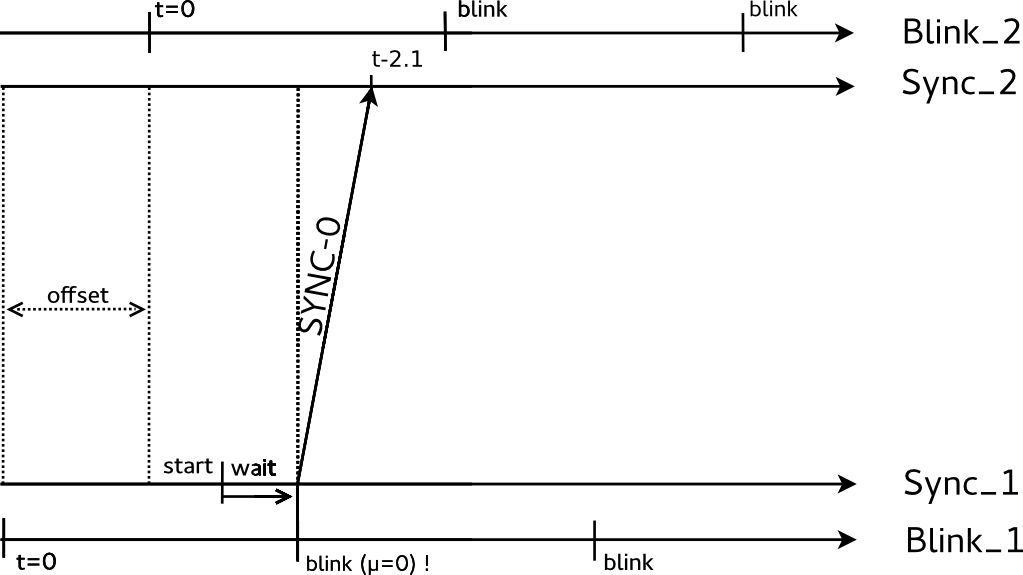
\includegraphics[scale=0.35]{assets/timesync-2.png}
    \end{center}
}
\frame{
    \frametitle{Time synchronization}
    \begin{center}
        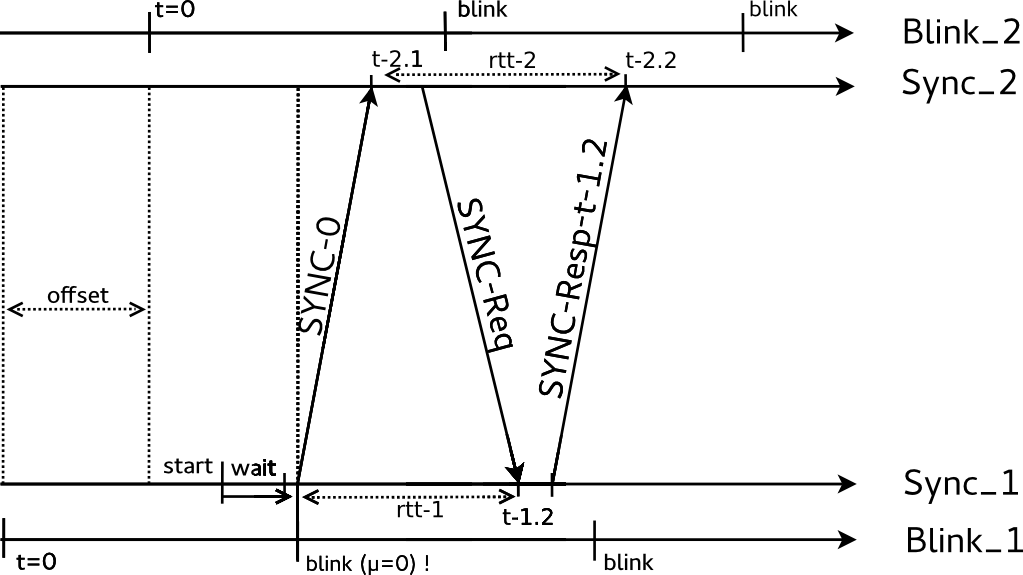
\includegraphics[scale=0.35]{assets/timesync-3.png}
    \end{center}
}
\frame{
    \frametitle{Time synchronization}
    \begin{center}
        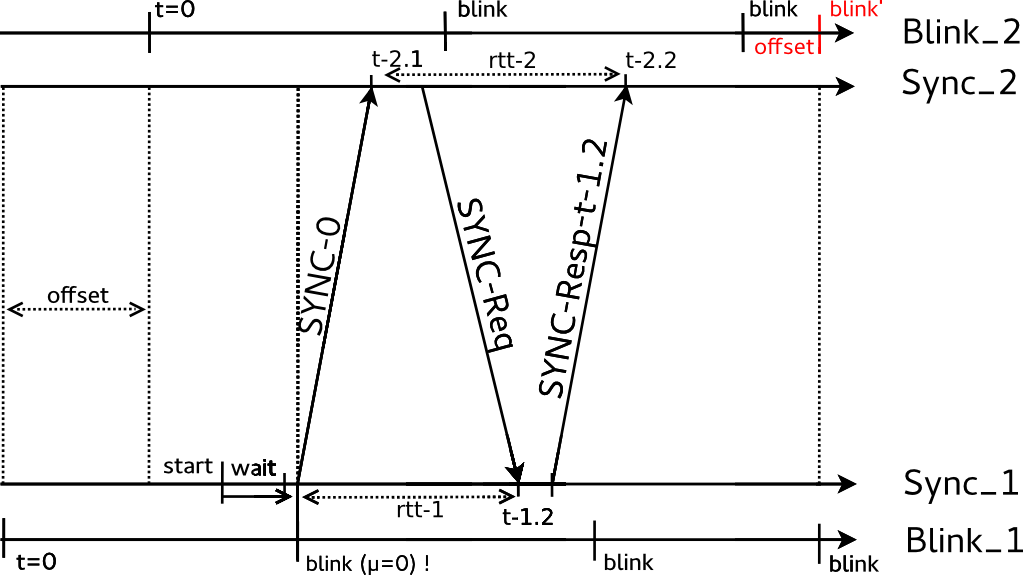
\includegraphics[scale=0.35]{assets/timesync-4.png}
    \end{center}
}


\begin{frame}[fragile]
  \frametitle{Time synchronization -- Code snippet}
  \begin{lstlisting}
    // If message comes from the leader (directly or indirectly),
    // record master and local timestamps and initiate ping-pong
    if (ts_src == leader_get_leader()) {

        t1_master = atoi(rcv_buffer + strlen(SYNC) + UID_LEN);
        // Get current time
        rtc_time(&tiv);
        gossip_send(node, DELAY_REQ_BUFFER, strlen(DELAY_REQ_BUFFER));
        t1_local = tiv.tv_usec;

    } else if (!strncmp(rcv_buffer, DELAYREQ, strlen(DELAYREQ))) {

        rtc_time(&tiv);
        sprintf(msg_buffer, "%s%s%s%s%08i", PREAMBLE, MSG, TS, DELAYRESP, tiv.tv_usec);
        gossip_send(node, msg_buffer, strlen(msg_buffer));

    } else if (!strncmp(rcv_buffer, DELAYRESP, strlen(DELAYRESP))) {

        rtc_time(&tiv);
        t2_local = tiv.tv_usec;
        t2_master = atoi(rcv_buffer + strlen(DELAYRESP));
        // Calculate offset
        offset = (t2_local > t1_local ? t2_local - t1_local : (1000000 - t1_local) + t2_local) / 2;
        master_offset = t1_local - offset > 0 ? t1_local - offset : 1000000 - t1_local;
        // Indicate that we have a trusted timestamp
        timesync_set_trusted(1);
    }
  \end{lstlisting}
\end{frame}

\frame{
  \huge{Issues}
}

\frame{
  \frametitle{Issues}
  \begin{itemize}
    \item RIOT is still work in progress
    \item We encountered several bugs, some of which were not previously
      known to the RIOT team
    \item Examples: Race conditions in hwtimer and vtimer, native
      implementation not float safe
    \item We communicated with the RIOT team during the project and
      contributed to issues
  \end{itemize}
}

\frame{
  \huge{Demo}
}

\frame{
  \frametitle{Demo}
  \begin{itemize}
    \item \textbf{Leader election: } If a node believes itself to be the
      leader, the green LED is on
    \item \textbf{Time synchronization: } The red LED blinks once
      a second -- the blinking is synchronized with the leader
  \end{itemize}
}

\frame{
  \huge{Integration into RIOT}
}

\frame{
  \frametitle{Integration into RIOT}
  \begin{itemize}
    \item The RIOT team has signaled that we can expect our code to be
      merged into the RIOT-OS/projects repository
    \item Just needs some cleanup and documentation
  \end{itemize}
}


\begin{frame}
 \frametitle{Discussion}
 \huge{Questions?}
\end{frame}

\end{document}
